\documentclass[output=paper,modfonts,nonflat]{langsci/langscibook}  
\title{Identification of multiword expressions: A fresh look at modelling and evaluation}
\shorttitlerunninghead{Identification of multiword expressions}
\author{Shiva Taslimipoor\affiliation{University of Wolverhampton}\and  Omid Rohanian\affiliation{University of Wolverhampton}\and  Ruslan Mitkov\affiliation{University of Wolverhampton}\lastand Afsaneh Fazly\affiliation{Thomson Reuters}
}
\abstract{Automatic identification of multiword expressions (MWEs) in running text has recently received much attention among researchers in computational linguistics. The wide range of reported results for the task in the literature prompted us to take a closer look at the algorithms and evaluation methods. For supervised classification of Verb+Noun expressions, we propose a context-based methodology in which we find word embeddings to be appropriate features. We discuss the importance of train and test corpus splitting in validating the results and present type-aware train and test splitting. Given our specialised data, we also discuss the benefits of framing the task as classification rather than tagging.}

\begin{document}

\maketitle
\label{TASLIMIPOOR-CHAPTER}

\section{Introduction} 

Ambiguity is a pervasive phenomenon in natural language. It starts from single words, and can propagate through larger linguistic constructs. Multiword expressions (MWEs) which are idiosyncratic combinations of two or more words, behave differently in their separate usages in running text. In natural language processing (NLP) tasks such as part-of-speech tagging, parsing and machine translation, these expressions should be treated either before the task \citep{nivre2004} or combined with the process \citep{constant2012evaluating,kordoni2011proceedings,nasr:acl:2015}. 

Examples of such expressions are: \textit{take action}, \textit{make sense} and \textit{set fire}.~\footnote{MWEs combine words from many different parts of speech. The pattern in our datasets is Verb+Noun, so all the examples in this chapter are of this kind.} 
MWEs are a recurring theme in any language with some sources estimating their number to be in the same range as single words \citep{Jac97} or even beyond \citep{Sag2002a}. Besides, new expressions come to languages on a regular basis. It is therefore not practically feasible to simply list MWEs in dictionaries or thesauri. 

More importantly, most idiomatic expressions can also have \isi{literal meaning} depending on context.
For instance consider the expression \textit{play games}. It is opaque with regards to its status as an MWE and depending on context could mean different things. For example in \textit{He went to play games online} it has a literal sense but is idiomatic in \textit{Don’t play games with me as I want an honest answer}. Resolving these cases is critically important in many NLP applications \citep{Katz06automaticidentification}. \cite{Katz06automaticidentification} framed the task as sense disambiguation. Tagging corpora for MWEs or token-based identification of MWEs\is{multiword expression!identification} is an example of a task where it is necessary to differentiate between idiomatic and literal usages of each expression type. 

Studies on MWEs can be divided into two main categories. One includes works regarding the canonical forms of expressions, their lexical properties and their potential to be considered as MWEs, namely type-based extraction of MWEs or MWE discovery; the other regards studies on tagging texts for the idiomatic usages of expressions, namely MWE tagging or token-based identification of MWEs. The former is a traditional approach which is of use to lexicographers as pointed in \cite{ramisch2014multiword}; the latter though, is more practical for NLP applications \citep{schneider-dimsum:2016}.

Although discovering canonical forms of multiword expressions is still an active research area \citep{salehi2013, farahmand2014}, recently there is a significant move towards automatic tagging of corpora for MWEs \citep{Schneider14b,constant2012evaluating}.

The focus of our study is token-based identification of MWEs, and we model it as a \isi{classification}, rather than a sequence labelling problem.\is{multiword expression!identification modelling}
To determine the idiomaticity of each Verb+Noun occurrence, we experiment with using solely context features without any sophisticated linguistic information. We do not exploit parsing, tagging or external lexicon-based information.
% EXPLAIN ABOUT OUR WORKSHOP PAPER AND the IMPROVEMET here
To discriminate between idiomatic and literal Verb+Noun expression tokens, we have proposed a context-based \isi{classification} approach expounded in detail in the previous publication~\citep{taslimipoor2017}. In this chapter, we build on this approach, experimenting with additional languages and several more sophisticated machine learning models. However, here we take a closer look at modelling and evaluation aiming at devising approaches that have more generalisation power and lead to less misleading results. We also conduct experiments to better demonstrate the suitability of framing our task as \isi{classification}.

For token-based identification of MWEs\is{multiword expression!identification}, there is a wide range of results in the literature reported as the state-of-the art: from F-score of 64\% with the DiMSUM dataset \citep{schneider-dimsum:2016} to 90\% \citep{W17-1717} for a dataset in the last PARSEME shared task\is{PARSEME!shared task} \citep{MWEWorkshop}.
We find that in order for the performance results not to be misleadingly high, the distribution of the tokens between train and test corpus, henceforth called \textsc{train and test splitting}, should be controlled. Failure to do so will result in a kind of overfitting which could be overlooked during evaluation. For instance, an expression like \textit{take advantage} is idiomatic consistently in all its usages in text. When different occurrences of this expression exist in both train and test corpus, the model memorises it from training data and predicts it very well in the test. Since such expressions are highly frequent, this memorisation helps the model to achieve erroneously high performance scores.

In the process of supervised identification of MWEs\is{multiword expression!identification}, we make observations with regards to the following: (1) the effect of train and test splitting of the tokens on generalisability of a model; (2) comparison between sequence labelling (tagging) and sequence \isi{classification}.

%\subsection{Motivation}
%For MWE \isi{identification} there is a wide range of results in the literature reported as the state-of-the art: from F-score of 64\% with the DiMSUM dataset \citep{schneider-dimsum:2016} to 90\% \citep{W17-1717} for a dataset in the last Parseme \isi{shared task} \citep{MWEWorkshop}.
%We find that in order for the performance results not to be misleadingly high, the distribution of the tokens between train and test should be controlled. Failure to do so will result in a kind of overfitting which could be overlooked during evaluation. For instance, an expression like \textit{take advantage} is idiomatic consistently in all its usages in text. When different occurrences of this expression exist in both train and test, the model memorises it from training data and predicts it very well in the test. Since such expressions are highly frequent, this memorisation helps the model to achieve erroneously high performance scores.  We propose a train and test splitting strategy in which all tokens of the same type are exclusively grouped into either train or test sets.

%Varieties of previous work on \isi{classification} or tagging MWEs, motivate us to more deeply look at the choice of the model based on the data. We argue that our task is naturally better suited to be defined as a \isi{classification} problem, and reformulating it as tagging results in reduced performance. 


\subsection{Literature review}

Identification of MWEs was shown to be effective in different NLP tasks, such as machine translation \citep{pal2011} and automatic parsing \citep{Constant2012}.
There exists a considerable body of work in the literature attempting to investigate lexical and syntactic properties of expressions to account for their potential for being MWEs \citep{ramisch2014multiword,baldwin2010multiword}. 
However, recently there has been a great attention given to identifying where exactly this potential takes effect by tagging a running text for each individual occurrence (token) of an expression \citep{Schneider14b,constant2012evaluating,Gharbieh2017}. 
Token-based identification of MWEs\is{multiword expression!identification} is effective in disambiguating between different behaviours of expressions in their individual usages. 
Evaluating all occurrences of expressions in the whole corpus of big size is not feasible. For this reason we have gathered a specialised dataset of concordances of particular expressions.

To the best of our knowledge, there are very few comprehensive tagged corpora for MWEs available, among which DiMSUM by \cite{schneider-dimsum:2016} is very recent and well-cited. This corpus was used in the SemEval (2016) shared task in Detecting Minimal Semantic Units and their Meanings (DiMSUM).
It is not particularly clear if the current methodologies applied to this corpus are capable of disambiguating between different usages of one specific canonical form.


\cite{cook2008vnc} prepared a dataset of \ili{English} Verb+Noun constructions, categorising expressions based on their idiomaticity and how consistent they behave in their different usages. \cite{fazly-cook-stevenson:2009:CL} have used that dataset for classifying Verb+Noun tokens into idiomatic or literal categories.

\cite{Katz06automaticidentification} used context features for identifying the idiomaticity\//\isi{non-compo\-sitionality} of MWEs in a different way. They represent different occurrences of an expression using LSA vectors and show that the vectors of the expressions in their idiomatic sense are very different from those of the same expressions in literal sense. Based on this observation they classify a test expression token depending on whether it is more similar to the idiomatic sense of the expression in training data or to the literal sense. % Can we try this for our data of group 2 ???

\cite{scholivet-ramisch:2017:MWE2017} recently tried to disambiguate a number of opaque \ili{French} expressions using their contexts. They proposed a tagging\is{sequence labelling} approach using unigram and bigram features of the word forms and their POS.
\cite{Qu+:2015a} found word embedding representation of the words in context very useful for tagging a text with MWEs. We also used word vector representations of the verb and noun components of the expression and the words in a window size of two on the right of the expression as features for classifying expressions as MWE or not. 

While most of the previous work on token-based identification of MWEs applied sequence tagging approaches using some kind of IOB labeling, \cite{legrand2016phrase} looked at the problem as \isi{classification}. They proposed a neural network based approach that learns fixed-size representations for arbitrary sized chunks which is able to classify these representations as MWE or not. They showed better performance in MWE identification over the CRF-based approach in \cite{constant2013}.


\subsection{Outline of the proposal}
\label{s:obs}

In almost all of the previous work on supervised modelling of MWE tokens, data is randomly split into train and test sets. %However, we have observed that by doing so the test data tends to overlap with the training data. 
In a random splitting, it is possible for occurrences of the same expression type to occur in both train and test sets. There are many instances where the expression almost always behaves idiomatically (e.g. \textit{take part}, \textit{make progress}) or literally (e.g. \textit{eat food}, \textit{give money}). In such cases a model learns every feature related to the POS and lemma form of the expression, and naturally can predict the correct tag for the expression perfectly in the test set (regardless of the expression being idiomatic or literal).  

Having observed this issue, for evaluation we propose and perform type-aware train and test splitting.\is{multiword expression!identification evaluation} To this end we divide expression types into train and test folds and gather all occurrences of each type into the same fold. This makes the predication rigorous, since the model performs cross-type learning.
One interesting study that considers cross-type learning of MWEs is the one by \cite{Fothergill2012}. However, they did not clearly explain %the motivation behind it and 
the general advantages and effects of cross-type \isi{classification} in evaluation. They used the approach in order to learn better features from specialised MWE resources. 

We propose type-aware splitting of the data as a supplementary benchmark for evaluating MWE identification\is{multiword expression!identification}. We design experiments to show the effectiveness of this kind of evaluation in assessing the generalisability of models.

Recent studies on token-based identification of MWEs are heading towards using structured sequence tagging\is{sequence labelling} models. The choice of the model based on the data is an important issue. Our data includes occurrences of specific Verb+Noun expressions with the context around them. This makes it possible to have sizeable datasets annotated for a specific type of MWE in order to have a extensive evaluation.  
We observe that our data cannot benefit from sequence tagging and a regular \isi{classification} approach can more reasonably model the data. We show better results from \isi{classification} over a tagging model. 
Other than traditional machine learning \isi{classification} approaches, we also propose a neural-network model by combining convolutional neural network and long short term memory models for identifying MWEs. Although some deep learning models have already been investigated for tagging MWEs by \citet{Gharbieh2017}, to the best of our knowledge this is the first time this approach has been applied for classifying MWE instances. 

We extensively discuss the following: 1) the division of data into train and test sets for evaluation and 2) the choice of model (\isi{classification} versus tagging)\is{multiword expression!identification modelling}\is{sequence labelling} based on the data.

\section{Context-based identification of MWEs}

In this study we use context features\is{feature} in a supervised environment to identify the idiomaticity of Verb+Noun expression tokens.\is{multiword expression!context-based identification} %The originality of this work lies on the observations covered in Section \ref{s:obs}. 
In order to construct context features, for our first set of experiments (\sectref{sec:res1}), given each occurrence of a Verb+Noun combination, we concatenate four different word vectors corresponding to the verb, noun, and their two following adjacent words while preserving the original order (following the previous work by \citealt{taslimipoor2017}). Concatenated word vectors are fed into different \isi{classification} models to be evaluated in terms of their performance.

The \isi{classification} algorithms that have been used are Logistic Regression (LR), Decision Trees (DT), Random Forest (RF), Multi Layer Perceptron (MLP) and Support Vector Machine (SVM). 
We also experimented with different neural network-based classification models. The best result is achieved with a combination of bidirectional Long Short-Term Memory network with a convolutional layer as a front-end (ConvNet+LSTM).  

For the second set of experiments (\sectref{sec:res2}), in which we compare Conditional Random Field (CRF) as a tagger with a simple Naive Bayes Classifier (NBC), we consider simple word forms of the verb, the noun, and the two words after as lexical context features.

We conducted our extensive experiments with \ili{Italian}. The experiments are augmented by applying the approach also for smaller data in \ili{Spanish} and \ili{English}.
%\textbf{Details about word2vec vectors, here?} 

\section{Experiments}

\subsection{Data}

We first experiment with two similarly formatted datasets in \ili{Italian} and \ili{Spanish} and later also on a %slightly different 
standard available dataset for \ili{English}.

For \ili{Italian}, our data includes a large set of concordances of Verb+Noun expressions.\footnote{The data as described in \cite{Taslimipoor2016} was gathered for four light verbs \textit{fare}, \textit{dare}, \textit{trovare} and \textit{prendre}. For some examples of expression instances refer to the same work.} % including the four verbs \text{},. 
Each item in the dataset is one concordance of a Verb+Noun expression and the whole item is annotated with 1 if the Verb+Noun inside is an MWE and with 0 otherwise.
The data as explained in \cite{Taslimipoor2016} was annotated by two native speakers with Kappa agreement measure of $0.65$. We resolved the disagreements by employing a third annotator who decided on most (but not all) cases of disagreements. This results in 20,030 concordances of 1,564 expression types. The \ili{Italian} data is very imbalanced and almost $70\%$ of the data is marked as MWE. To resolve this issue, we ignore the $15$ most frequent expression types which are exclusively marked as MWE and also the expressions with frequency lower than $3$. As a result we run the experiments on 18,540 concordances of $940$ expression types.

For \ili{Spanish}, we extracted concordances of Verb+Noun expressions in the same way using SketchEngine \citep{kilgarriff2004}.\footnote{For \ili{Spanish}, we focused on four light verbs \textit{tener}, \textit{hacer}, \textit{dar} and \textit{tomar}, similar to the ones we use for \ili{Italian}.} After ignoring the concordances for five most frequent expressions, $3,918$ usages were marked by two native speakers. The Kappa \isi{inter-annotator agreement} was $0.55$. Having seen the observed agreement of 0.79, we ignored all cases of disagreements and considered only the concordances on which both annotators agreed. 
This results in $3,090$ concordances of $747$ expression types.  

For \ili{English}, we employ a standard dataset called VNC-tokens prepared by \cite{cook2008vnc}.\footnote{The dataset is available in \url{https://sourceforge.net/projects/multiword/files/MWE_resources/20110627/}} The dataset is a benchmark for \ili{English} verb-noun idiomatic expressions\is{verbal multiword expression!verb-noun} and was used for identifying MWE tokens in a number of previous studies such as \cite{fazly-cook-stevenson:2009:CL} and \cite{salton2016acl}.
The dataset includes sentences from the BNC corpus including occurrences of Verb+Noun expressions and is suitable for our task since it contains expressions with both skewed and balanced behaviour in being literal or idiomatic. 
Rather than concordances, it includes sentences from BNC containing occurrences of Verb+Noun expressions.
%Unlike in \ili{Italian} and \ili{Spanish} where data collection was restricted to four specific verbs and all occurrences of those verbs with any following noun were extracted, in the case of 
Two \ili{English} native speakers selected the expression types based on whether they have the potential for occurring in both idiomatic or literal senses. Although this dataset is slightly different from our \ili{Italian} and \ili{Spanish} data (which are extracted randomly), it has the same favourable pattern of different occurrences of same expression types that can be split into train and test. We find it interesting to investigate our observations on a differently gathered but standard dataset. 
The Verb+Nouns in this dataset are not necessarily continuous.
We ignore the cases where the Verb+Noun occurs in passive form and the ones that the annotators were unsure of and this results in $2,499$ sentences consisting of Verb+Noun expressions. The statistics of the data for all three languages are reported in \tabref{tab:data}.

\begin{table}[!ht]
\small
\caption{Distribution of the data}
\label{tab:data}
 \begin{tabular}{lccc} 
  \lsptoprule
    & Italian & Spanish & English  \\
  \midrule
   Expression types & 940 & 747 & 53 \\
   Expression tokens & 18,540 & 3,090 & 2,499  \\
   MWE tokens  & 10,804 (58.27\%) & 2,094 (66.57\%) & 1,981 (79.27\%)  \\
  \lspbottomrule
 \end{tabular}
\end{table}


For all the three datasets, we consider the same context words as features for \isi{classification}: we extract the vectors of the verb, noun and the two words after the noun. 

\subsection{Evaluation}

In all cases classifier performance was measured using 10-fold cross-validation.

\subsubsection{Standard splitting of data into train and test}
In the standard method of performing cross-validation, the whole data is randomly divided into $k$ folds and then the model is repeatedly trained on the data of $k-1$ folds and tested on the data of the remaining fold. The result is averaged among $k$ different iterations. In our task, we find the result of this evaluation misleading\is{multiword expression!identification evaluation}, since the repetition of the same expression in both train and test partitions helps the model to predict those specific types of expressions well, while the model might not work for new unseen expressions in test. Even stratified cross-validation suffers from the same kind of overfitting. In standard stratified cross-validation, imbalance is coped with by controlling the distribution of labels alone, so that all folds have the same distribution of labels. Similar to standard cross-validation, this method is not informed about the idiosyncratic distribution of types and tokens.

Therefore, these methods of evaluation cannot precisely reflect the effectiveness of the model or features and show better results for models that are more prone to overfitting. It is not particularly clear from this kind of evaluation if a good performing model could be generalised to unseen expressions and also to ambiguous expressions that have balanced distribution of occurrences as literal or idiomatic.
We show the performance computed using this type of evaluation for different classifiers in \tabref{tab:regular}.


\subsubsection{Type-aware splitting and evaluation}


We perform a custom cross-validation by splitting the expression occurrences into different folds considering their types/canonical forms\is{multiword expression!identification evaluation}. We split the expression types into $k$ groups and all the occurrences of the expressions in the $k^{th}$ group goes into the $k^{th}$ fold. 
This method ensures that the model performs cross-type learning and generalises to tokens from unseen types in the test fold. In other words, the model is learning the features and general patterns and does not overfit on highly recurrent token occurrences.\is{multiword expression!type-aware classification}
%with consistent behaviour
The results for all classifiers evaluated using this approach is reported in \tabref{tab:typeaware}.

%\subsection{Type-specialised evaluation?? (Maybe I should try more by larger context)}
%In this type of evaluation, we consider a specific type of expression which has a balanced distribution of idiomatic or literal occurrences. We split the concordances of the target expression type into train and test partitions and evaluate the best of our supervised classifiers on it. This kind of evaluation is particularly useful to show the performance of the model in disambiguating between different occurrences of an expression type.
%\textbf{Our model has been tried on different types of expressions and does not show any good performance for any.}

\section{Results}

In this section, first a comparison of several classifiers using different train and test splitting methods is reported; then we present experiments using sequence tagging for identifying MWEs; and finally, the effectiveness of neural network-based \isi{word embeddings} compared with count-based representations was analysed using one of the best classifiers.
%the classifiers for discriminating between different usages of expressions has been analysed. 

\subsection{Regular and type-aware evaluation}
\label{sec:res1}
Evaluation performances\is{multiword expression!identification evaluation} for all classifiers using two different kinds of train and test splitting, namely regular (random) and our proposed type-aware\is{multiword expression!type-aware evaluation}, are reported in \tabref{tab:regular} and \tabref{tab:typeaware}.
The columns of the tables represent the results for \ili{Italian} (IT), \ili{Spanish} (ES) and \ili{English} (EN).
All traditional classifiers in this experiment use the same vectorised context features. 
The word vectors used in this study are available online.\footnote{\url{http://hlt.isti.cnr.it/wordembeddings/} for Italian and \url{https://github.com/Kyubyong/wordvectors} for Spanish} The generated \ili{Italian} and \ili{Spanish} \isi{word embeddings} applied Gensim’s skipgram word2vec model with the window size of 10 to extract vectors of size 300.
%However, for \ili{English}, since we have got better results with vectors from simple count-based embeddings as explained in Section \ref{s:wv-res}, those vectors are used instead of word2vec.
For \ili{English} we use \isi{word embeddings} of the same dimension trained using Glove \citep{pennington2014glove} algorithm available via spaCy.\footnote{\url{https://spacy.io/docs/usage/word-vectors-similarities}}

We also report the results from a more sophisticated neural network based architecture comprising of a BiLSTM with an additional convolutional layer as a front-end (ConvNet+LSTM). For this architecture the context window size is $2$ (two words before and two words after the Verb+Noun expression).\footnote{The difference in results were negligible when considering only the two context words on the right.} Implementation details of these experiments can be found at \url{https://github.com/shivaat/VN-tokens-clf}. 

\begin{table}[!ht]
\caption{Regular evaluation results: accuracy (standard deviation)}
\label{tab:regular}
 \begin{tabular}{lccc} 
  \lsptoprule
   Classifiers & IT & ES & EN  \\
  \midrule
   Majority Baseline & 0.5827 & 0.6657 & 0.7927\\
   LR & 0.8869 (0.007)  & 0.9129 (0.011) & 0.8651 (0.020)  \\
   %LDA & 0.8464 (0.118) & 0.7560 (0.03) & 0.8491 (0.017) \\
   DT  & 0.8905 (0.008) & 0.9065 (0.017) &  0.8799 (0.018) \\
   RF & 0.9218 (0.005) & 0.9337 (0.019)  &  0.9024 (0.017)\\
   MLP & 0.9069 (0.006) & 0.933 (0.009) &  0.9056 (0.016) \\
   %KNN & 0.8474 (0.005) & 0.7129 (0.02) & 0.8920 (0.025) \\
   %GB & 0.9140 (0.006) & 0.7940 (0.02) & 0.8872 (0.022) \\
   SVM  & 0.9116 (0.005) & 0.9207 (0.009) & 0.7927 (0.021) \\
   ConvNet+LSTM  & \textbf{0.9220 (0.007)} & \textbf{0.9668 (0.01)} & \textbf{0.8860 (0.024)} \\
  \lspbottomrule
 \end{tabular}
\end{table}


\begin{table}[!ht]
\caption{Type-aware evaluation results: accuracy (standard deviation)}
\label{tab:typeaware}
 \begin{tabular}{lccc} 
  \lsptoprule
  Classifiers & IT & ES & EN  \\
  \midrule
   Majority Baseline & 0.5827 & 0.6657 & 0.7927\\
   LR & 0.6909 (0.06)  & 0.8178 (0.074) & 0.8092 (0.149)  \\
   %LDA & 0.6778 (0.06) & 0.6502 (0.07) & 0.7797 (0.079) \\
   DT  & 0.6048 (0.03) & 0.7483 (0.078) & 0.6327 (0.128) \\
   RF & 0.6337 (0.08) & 0.7604 (0.097) & 0.7321 (0.19) \\
   MLP  & 0.7053 (0.06) & 0.8319 (0.086) & 0.7294 (0.169) \\
   %KNN  & 0.6829 (0.07) & 0.6499 (0.05) & 0.7498 (0.063) \\
   %GB & 0.6976 (0.08) & 0.7111 (0.05) & 0.7731 (0.099) \\
   SVM  & \textbf{0.7369 (0.07)} & 0.8460 (0.093) & 0.8062 (0.152) \\
   ConvNet+LSTM  & 0.6601 (0.053) & \textbf{0.8681 (0.072)} & \textbf{0.8112 (0.106)} \\
  \lspbottomrule
 \end{tabular}
\end{table}

Different classifiers show high performance with not much difference using regular cross-validation in which tokens are distributed into separate folds regardless of their types (\tabref{tab:regular}). ConvNet+LSTM, in particular, performs the best, %exceptionally well, 
which we believe is the result of overfitting arising from this method of train and test splitting. 
However, we can see notable differences between classifiers in \tabref{tab:typeaware} where we cross validate in a way that no same expression type occurs in both train and test partitions. %These results are similar both for \ili{Italian} and \ili{Spanish}.

In the case of cross-type learning (\tabref{tab:typeaware}), the SVM classifier showed the best results in identifying MWEs using vectorised context features for \ili{Italian}, and close to the second best for \ili{Spanish} and \ili{English} data for which ConvNet+ ~~~~~~~LSTM is the best. The performance of this classifier is followed by that of MLP and LR for both \ili{Italian} and \ili{Spanish}. For \ili{English} the results of SVM and LR are comparable. Computed performance for other classifiers like DT and RF dropped sharply when we use our type-aware cross-validation.
This is also the case for ConvNet+LSTM for \ili{Italian} data.
 %ConvNet+LSTM has the most drastic drop in performance across the tables. 
This experiment determines how well a classifier can generalise among different expression types. SVM and LR in particular are shown to be fairly suitable for cross-type identification of MWEs. MLP also performs relatively well overall. 

As for the \ili{English} data it is worth noting that the VNC data is very imbalanced with the majority baseline of $0.7927$ which is difficult to beat by classifiers. 


%We also perform some smaller scale experiments with the VNC-tokens.  

\subsection{Sequence classification versus sequence tagging}
\label{sec:res2}
The experimental data in this study can be perfectly processed with standard \isi{classification} approach, since the goal is to predict idiomaticity of an expression in a given context. However, \cite{scholivet-ramisch:2017:MWE2017} modelled such a data with sequence tagging\is{sequence labelling}. We believe that since not all the words in a sequences are going to be tagged, MWE identification\is{multiword expression!identification} using such a data cannot benefit from sequence labelling. 
We applied sequence tagging on the data to properly investigate the effects. Specifically, simple Naive Bayes Classifier (NBC) was considered as a simple sequence \isi{classification} methodology and Conditional Random Field (CRF) was used as the sequence tagging approach. Both of the models use simple nominal features: the verb, the noun, and the two words after the noun.\footnote{The features are the surface text occurrences of these words.} The results are reported in \tabref{tab:seqLabel} in terms of accuracy.

\begin{table}[!ht]
\small
\caption{Performance of sequence classification versus sequence tagging}
\label{tab:seqLabel}
 \begin{tabular}{lccccccc} 
  \lsptoprule

   & \multicolumn{3}{c}{regular}  & & \multicolumn{3}{c}{type-aware %\footnote{These ones are very variant in different runs (depending on the distribution of types in different folds).}
   } \\
   & \multicolumn{3}{c}{cross-validation} & & \multicolumn{3}{c}{cross-validation} \\
   \midrule
   & IT & ES & EN & & IT & ES & EN \\
 NBC  &  0.9504 & 0.9601 & 0.8560 & & 0.7291 & 0.7298 & 0.6013 \\
% (with actual 4 words)  &  &      \\
 %\hline
 CRF  &  0.9165 & 0.9142 & 0.8176 & & 0.6447 & 0.7199 & 0.6848 \\
  \lspbottomrule
 \end{tabular}
\end{table}

As can be seen in \tabref{tab:seqLabel}, CRF cannot even beat the simple naive bayes classifier except in the case of \ili{English} data (when we apply cross-type learning). This is because our data is naturally suited for sequence \isi{classification} and cannot benefit from sequence labelling models.\is{multiword expression!identification modelling}

\subsection{Effectiveness of word embedding representation}
\label{s:wv-res}
To specifically show the effectiveness of neural network-based embeddings\is{word embeddings} for the classifiers to identify Verb+Noun MWEs, we performed an experiment using sparse bag-of-words count vectors with tf-idf weighting. In this case each sentence is considered as a collection of words, disregarding any word order. The sparse vector for each word is constructed based on its occurrence in different sentences. Each entry of the vector is weighted by $tf$ (the word frequency) $*$ $idf$ (the inverse of frequency of the sentences containing the word). Similar to previous experiments, we feed the vectors to a Multi Layer Perceptron (MLP) which works reasonably well compared to other classifiers based on the previous experiment. Note that the execution time for the best performing model, SVM, is almost 5 times that of MLP which makes it inefficient in comparison. The results of this comparison can be seen at \tabref{tab:wv}.


\begin{table}[!ht]
\small
\caption{The accuracy of MLP in identifying Verb+Noun MWEs using word2vec and count-based embedding}
\label{tab:wv}
 \begin{tabular}{cccc}
  \lsptoprule
  & \multicolumn{3}{c}{Accuracy (std.)} \\
  & IT & ES & EN \\
  \midrule
  MLP with count based embedding & 0.6504 (0.0354) & 0.7851 (0.042)  & 0.7002 (0.099) \\
  MLP with word2vec & 0.7053 (0.06) &   0.8319 (0.086) & 0.7294 (0.169) \\
  \lspbottomrule
 \end{tabular}
\end{table}

The results in \tabref{tab:wv} show the improvement in performance when using \isi{word embeddings} rather than the vanilla count-based vectors for all three languages (although less significant for \ili{English}). 
 
\section{Discussion}

In order to understand the argument behind type-aware evaluation\is{multiword expression!type-aware evaluation} and decide its applicability, we have to look at the distribution of data points. In the \ili{Italian} data, for instance, the majority of data points belong to MWE types whose tokens occur invariably as idiomatic or literal only. In other words, if we plot the distribution of tokens with regards to the degree of idiomaticity of their corresponding types, we would see a skewed distribution (even after ignoring the 15th most frequent expressions), where only a smaller portion of tokens belong to MWE types whose usages can be fluid between literal and idiomatic. In such a scenario, a model easily overfits on the majority of the data, where labels were assigned invariably. However, this skewedness is not necessarily reflected in the distribution of MWE labels, as we might see a relatively balanced distribution of literal and idiomatic labels. This means there might be no severe class imbalance in the dataset, but within-class imbalance \citep{ali2015classification}.

\begin{figure}[!htb]
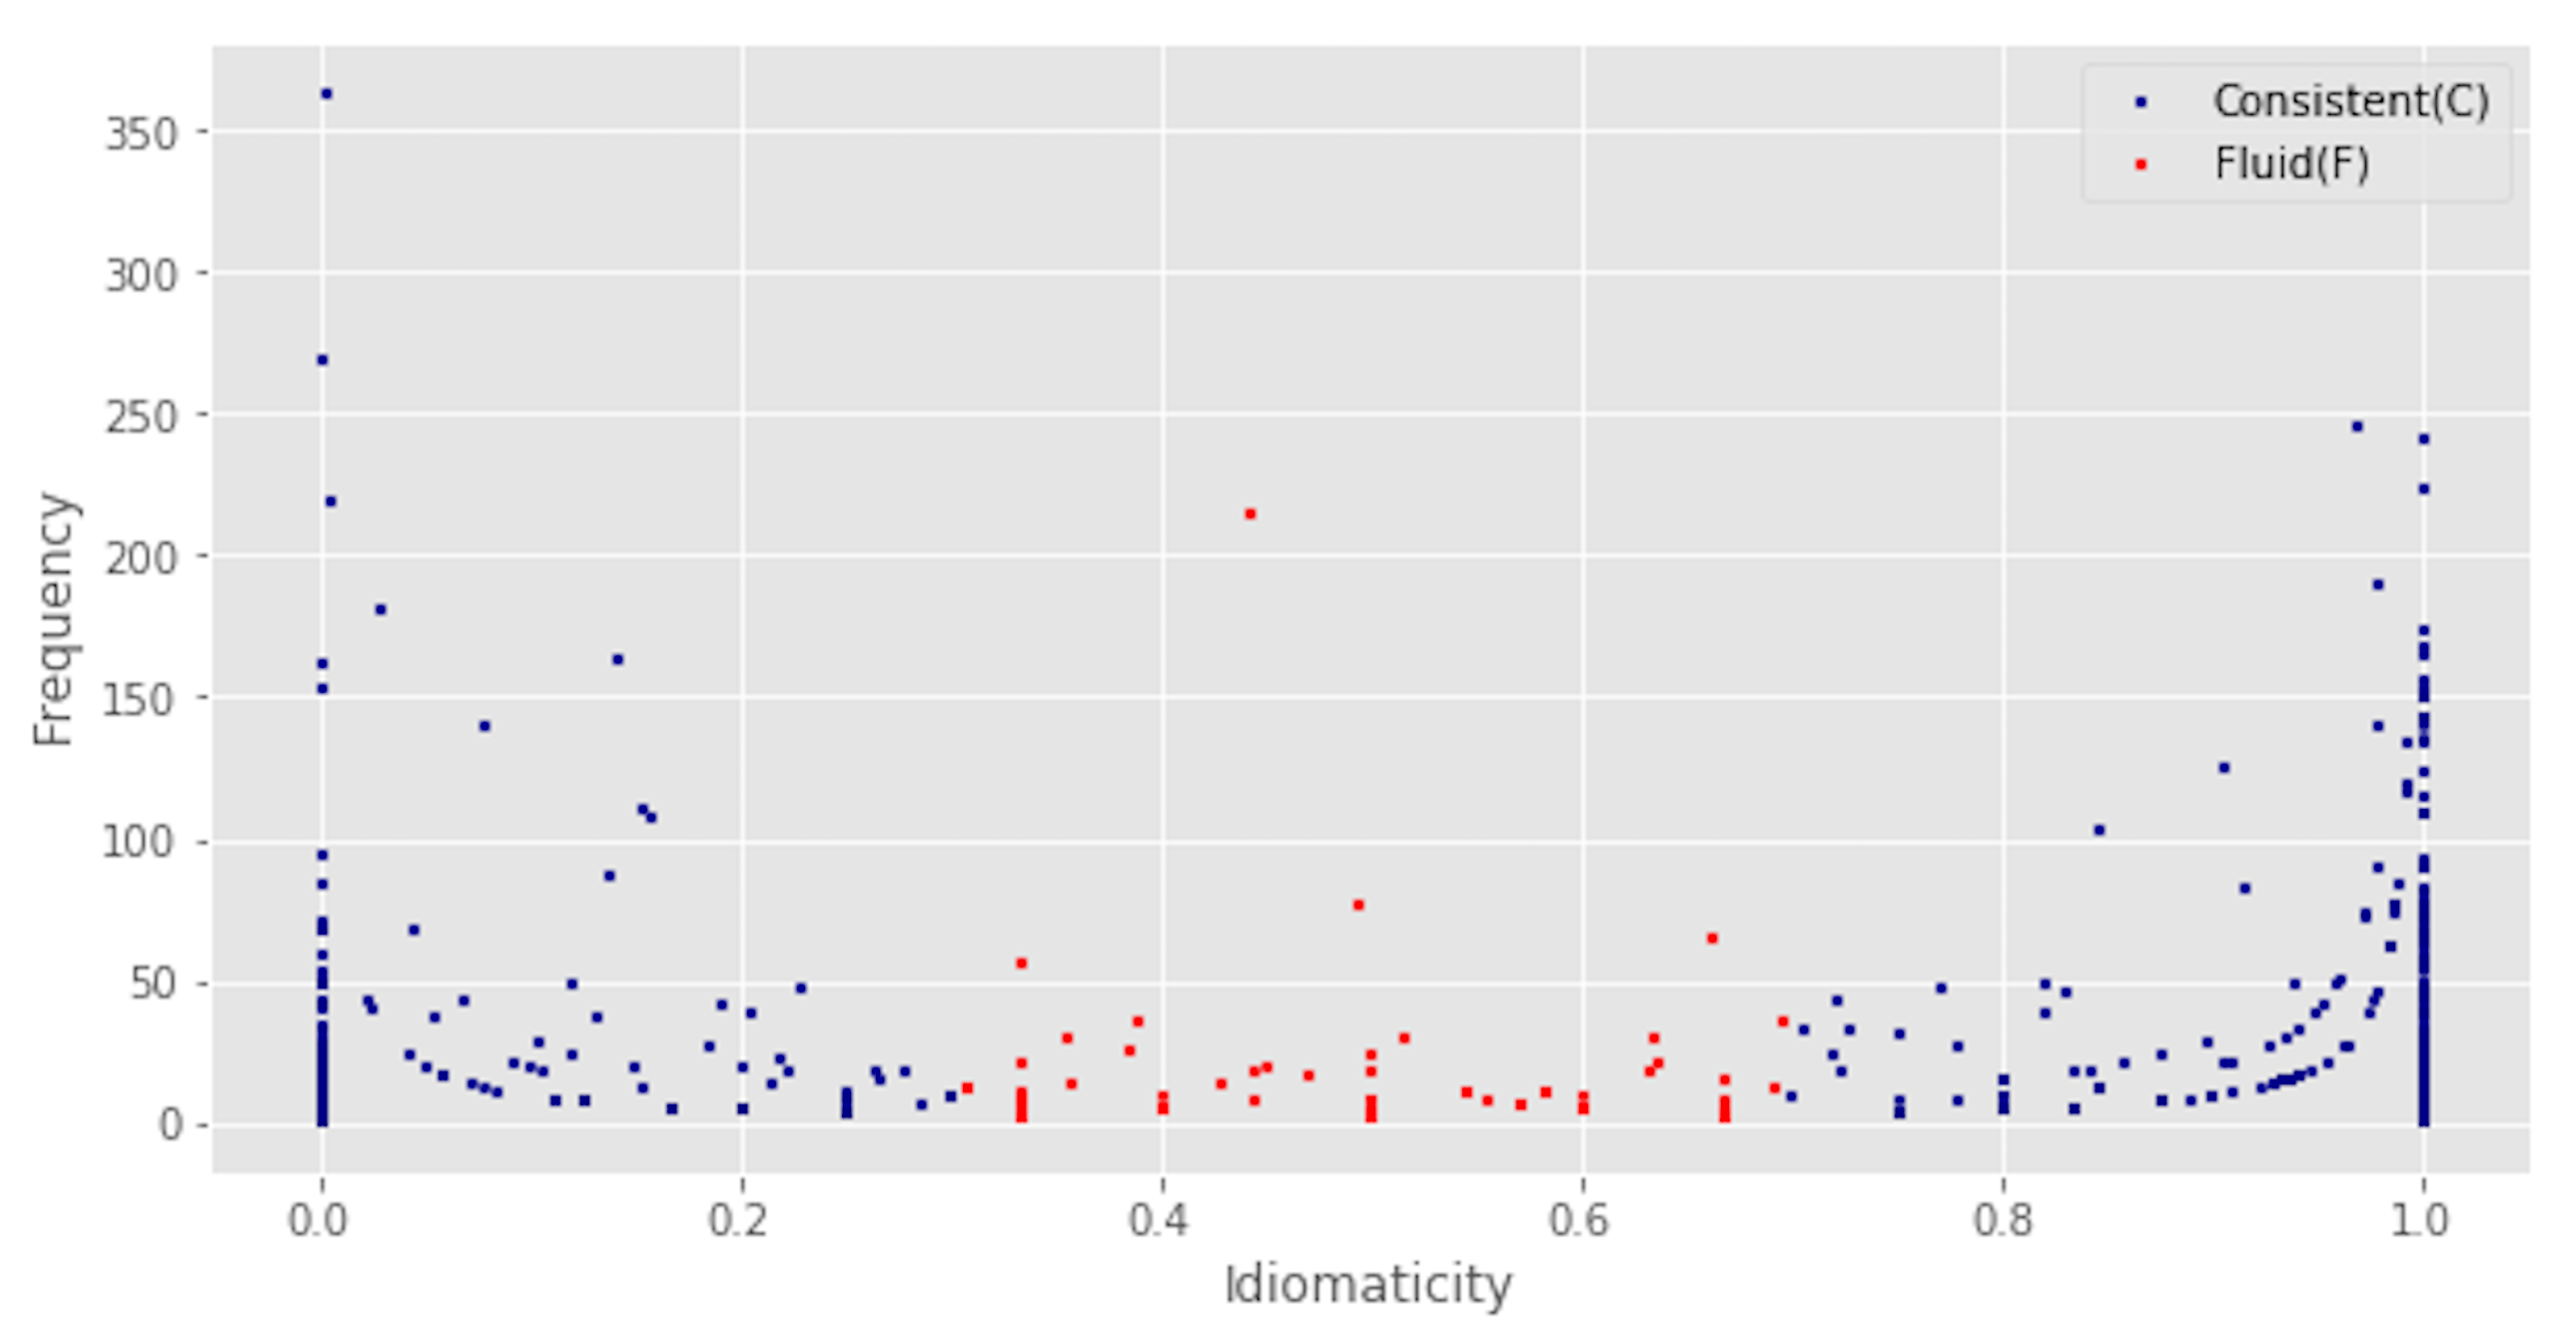
\includegraphics[scale=0.45]{figures/data_imbalance.png} 
\caption{Distribution of expression types.}
\label{fig:data}
\end{figure}


To illustrate the point, we operationalise two categories for MWE types, namely Consistent (C) and Fluid (F). Those types whose tokens occur more than 70\% or less than 30\% of the time as only literal or idiomatic are tagged as C, and the rest are considered F. Accordingly, %if we look at the labels 1, and 0 in the dataset separately we can trace back what categories the tokens in each class belong to. 
\figref{fig:data} shows the distribution of the expression types with regards to the behavior of their corresponding tokens. As can be seen, the majority of expressions with higher token frequencies are from the sub-class C. 
%there is a huge within-class imbalance, as the majority of the tokens in both classes are from types categorized as C.  
For this reason, evaluation using a vanilla cross validation or even stratified cross validation would not provide us with reliable results, since splitting of train and test disregards the within-class imbalance inherent in the data. 

Since this is the case with data in real world, we propose type-aware train and test splitting as a supplementary approach for modelling the data and evaluating the results. This way, we make sure that a model has the best ability for generalisation, learns general properties for MWEs and is not merely based on memorising the words that construct MWEs.% when they occur together.

It is worth noting that we did not used any linguistic or lexical features and we expect vector representation of context to be generalisable enough. Even with these generalisable features we observe substantial differences between regular and type-aware cross-validation.
A proper method for train and test splitting is even more essential to validate the evaluation when a model trains on more exact features such as lexical ones.

With regards to previous data and models for MWEs, DiMSUM is one of the most noteworthy shared tasks.
DiMSUM includes a recent tagged corpus for MWEs with a fairly small size of $4,799$ sentences in train and $1,000$ in test, including all types of MWEs. With such limited data, we observed only a few number of expressions of the form Verb+Noun occurring in both train and test. To give an example, with a selection of 6 most frequent light verbs, all their combinations with nouns are only 13 occurrences in the test data, out of which only 3 are MWEs. There are no repeated occurrences of these cases in both train and test data. Therefore, we believe that this data inherently does not lead to misleading results. In other words, a model that works well on this data could be fairly generalised.

\cite{Gharbieh2017} showed better performance when using deep neural network models compared with traditional machine learning on DiMSUM. However, in our experiment of \isi{type-aware classification}, SVM performed the best, even outperforming LSTM and ConvNet and their combinations for \ili{Italian} and \ili{Spanish}.
Since neither DiMSUM nor our data is big enough for a proper analysis with deep learning, more studies are required to find the most effective model to identify MWEs.

Another data for token-based identification of MWEs\is{multiword expression!identification} in \ili{English} that we also used in this study is VNC-tokens \citep{cook2008vnc}. One advantage of this corpus is that the data is particularly gathered for the task of disambiguation between idiomatic and literal usages of expressions. Before the annotation, they selected only the expressions that have the potential for occurring in both idiomatic and literal senses. 
Although we did not follow the initial development splitting of the data for this study (i.e. we followed our proposed way of splitting the data into train and test),
the development and test splitting of this data is type-aware. Therefore, an experiment with this data, is able to truly measure generalisation. % Although Gharbieh et al. (2016) have performed leave-one-out approach for evaluation on the whole Dev or Test and somewhat ignored that the results might be good because of overfitting for expressions with more consistent behaviour.

In PARSEME shared task \citep{MWEWorkshop}, which features the most recent multi-lingual data for MWEs, \cite{maldonado2017} presented statistics on the percentage of previously seen data in test sets of all languages (i.e. proportion of MWE instances in the test set that were seen also in the training set). The correlation between these percentages and the results stress the need for proper train and test splitting. \citetv{Maldonadotv}  further discuss the characteristics of the shared task data and report the performance results of the systems on seen and un-seen data separately.  
The experiments with the data for the Parseme shared task, which is also discussed in \citetv{Savarytv}, would definitely benefit from such type-aware train and test splitting.

\section{Conclusions}
In this study, we explored a context-based classification method for identification of Verb+Noun expressions. We employed word embedding to represent context features for MWEs. We evaluated the methodology using type-aware cross-validation and discussed its effectiveness compared with standard evaluation. We argue that only this proposed method properly accounts for the generalisability of a model. We also showed that our data (and similar ones) for this task cannot benefit from structured sequence tagging models.

The effectiveness of word embeddings as context features for identifying MWEs should be examined in more detail with datasets of larger size and with more sophisticated embeddings that consider linguistic features. We would also like to analyse the effect of our proposed approach on unseen and less frequent data. 


\section*{Acknowledgements}
The authors would like to thank Manuela Cherchi, Anna Desantis, Martina Cotella, Andrea Silvestre and Alondra Nava Zea for their help in annotations.
%\ea
%\gll dit          is           een             voorbeeld.\\
%     \textsc{dem} \textsc{cop} \textsc{indef}  example\\
%\glt `This is an example.'
%\z

\section*{Abbreviations}


\begin{tabularx}{.52\textwidth}{ll}
 \textsc{b}i\textsc{lstm}  & bi-directional long \\ 
 & short-term memory  \\
\textsc{crf}  & conditional random field  \\
\textsc{ConvN}et  & convolutional neural network \\
\textsc{dt}  & decision tree  \\
\textsc{iob}  & inside-outside-beginning  \\
\textsc{lsa}  & Latent Semantic Analysis  \\
\textsc{lr}  & logistic regression  \\
\end{tabularx}
\begin{tabularx}{.48\textwidth}{ll}
\textsc{lstm}  & long short-term memory \\
\textsc{mlp}   & multi-layer perceptron \\
\textsc{mwe} & multiword expression \\
\textsc{nbc}  & naive Bayes classifier  \\
\textsc{nlp} & Natural Language Processing  \\
\textsc{pos} & part of speech  \\
\textsc{rf}  & random forest \\
\textsc{svm}  & support vector machine \\
\end{tabularx}


%\printbibliography
{\sloppy
\printbibliography[heading=subbibliography,notkeyword=this]
}

\end{document}
